%%%%%%%%%%%%%%%%%%%%%%%%%%%%%%%%%%%%%%%%%%%%%%%%%%%%%%%%%%%%%%%%%%%%%%%%%%%
% * <sonya.hanson@choderalab.org> 2015-04-23T18:56:00.248Z:
%
% 
%
% HEADER: DON'T EDIT THIS!
%%%%%%%%%%%%%%%%%%%%%%%%%%%%%%%%%%%%%%%%%%%%%%%%%%%%%%%%%%%%%%%%%%%%%%%%%%%
% ^ <sonya.hanson@choderalab.org> 2015-04-23T18:57:46.938Z.
% But why not?

\documentclass[11pt]{article}

\title{ Advancing predictive physical modeling through focused development of model systems to drive new modeling innovations}

\usepackage[top=0.5in, bottom=0.5in, left=0.5in, right=0.5in]{geometry}
\usepackage{helvet}
\usepackage{url} % hypderref?
\usepackage{graphicx}
\graphicspath{{figures/}} % The figures are in a figures/ subdirectory.
\renewcommand{\familydefault}{\sfdefault}
\pagestyle{empty}
%\pagestyle{plain}

% Fancy page-width tables
\usepackage{tabularx}

% Use a package for framed boxes
\usepackage{mdframed}

\usepackage[T1]{fontenc}
\usepackage{amssymb}


\usepackage{setspace}
\usepackage{microtype}

\usepackage{amsfonts}
\usepackage{amsmath}

\usepackage{floatrow}

\usepackage[normalem]{ulem} % for nci.bst

\usepackage{sidecap}
\usepackage[abs]{overpic}
\usepackage{wrapfig}

%\usepackage[round,authoryear]{natbib}
\usepackage{cite}
%\setlength{\bibsep}{0.00in}

\usepackage{hyperref}
\hypersetup{colorlinks=true, urlcolor=black, citecolor=black, linkcolor=black}

\newcommand{\doi}[1]{\href{http://dx.doi.org/#1}{doi:#1}}

\newcommand{\ac}[1]{{\sc \lowercase{#1}}}

\renewcommand{\baselinestretch}{.93}
%\renewcommand{\baselinestretch}{.90}
\usepackage{wrapfig} 

\usepackage{bibspacing}
\setlength{\bibspacing}{\baselineskip}


\graphicspath{{figs/}}

\makeatletter

\newcommand{\captionfonts}{\footnotesize}

\makeatletter  % Allow the use of @ in command names
\long\def\@makecaption#1#2{%
  \vskip\abovecaptionskip
  \sbox\@tempboxa{{\captionfonts #1: #2}}%
  \ifdim \wd\@tempboxa >\hsize
    {\captionfonts #1. #2\par}
  \else
    \hbox to\hsize{\hfil\box\@tempboxa\hfil}%
  \fi
  \vskip\belowcaptionskip}      
\makeatother

\renewcommand{\figurename}{{\bf Figure}}

% Page numbering.
%\pagestyle{plain}
%\pagenumbering{arabic}

\setlength{\abovecaptionskip}{-5pt}

\makeatother

\renewcommand{\refname}{Bibliography and References Cited}

\setlength{\parindent}{0pt} % Don't indent first line
%\setlength{\parskip}{1ex plus 0.5ex minus 0.2ex} % Add some space between paragraphs
\setlength{\parskip}{0.8ex} % Add some space between paragraphs

\begin{document}

%======================================
% CITE OUR REFS FIRST
%\phantom{
%\cite{mobley-chodera-dill:2006:jcp:orientation-restraints,mobley-chodera-dill:2007:jctc:confine-and-release,shirts-mobley-chodera-pande:2007:jpcb:dispersion-corrections,chodera:jcp:2007,shirts-mobley-chodera:2007:annu-rep-comput-chem:prime-time,shirts-chodera:jcp:2008:mbar,ncmc,chodera-shirts:jcp:2011:gibbs,chodera:curr-opin-struct-biol:2011:drug-discovery,chodera-shirts:jcamd:2013:yank}
%\cite{gunner:biophys-j:1997:mcce,gunner:bba:2000:proton-electron-transfer,gunner:biophys-j:2002:mcce,gunner:j-comput-chem:2009:mcce2,gunner:jmb:2009:mcce2-hsa,gunner:proteins:2010:reaction-center,dutton:biochem:1994:photosynthetic-reaction-center,gunner:proteins:2010:reaction-center,gunner:photosynth-res:2013:photosynthetic-reaction-center,gunner:bba:2000:proton-electron-transfer,gunner:j-comput-chem:2009:mcce2,nielsen-gunner-garciamoreno:proteins:2011:pka-cooperative,stanton-houk:jctc:2008:benchmarking-pka-prediction}
%}

%%%%%%%%%%%%%%%%%%%%%%%%%%%%%%%%%%%%%%%%%%%%%%%%%%%%%%%%%%%%%%%%%%%%%%%%%%%
% SPECIFIC AIMS
%%%%%%%%%%%%%%%%%%%%%%%%%%%%%%%%%%%%%%%%%%%%%%%%%%%%%%%%%%%%%%%%%%%%%%%%%%%

%{\large \bf SPECIFIC AIMS}

%\eject

%%%%%%%%%%%%%%%%%%%%%%%%%%%%%%%%%%%%%%%%%%%%%%%%%%%%%%%%%%%%%%%%%%%%%%%%%%%
% SIGNIFICANCE
%%%%%%%%%%%%%%%%%%%%%%%%%%%%%%%%%%%%%%%%%%%%%%%%%%%%%%%%%%%%%%%%%%%%%%%%%%%


%NEED TO CAREFULLY CONSIDER GRAPHICS -- SOMETHING ON SIGNIFICANCE?

{\large \bf SIGNIFICANCE}
%2 pages

{\color{red}[JDC: In general, can we break things up more with subsection headings or bold lead phrases? The first page is fine, but beyond this, it may be tiresome to just have a ``wall of text''.]}
%Should I be adding boldface mini-summaries here to make it easier to skim?

%Promise of physical methods, how they could transform drug discovery and the design of new small molecules for chemical biology
% (If space permits here we will allude also to how this could help with broader areas too such as engineering of biologics)
Physical methods are poised to transform drug discovery and chemical biology by enabling true molecular design. 
While modeling work is already used extensively in drug discovery, its main role at present is to aid with idea generation or to filter large libraries of compounds for screening. 
Instead, we imagine using computational techniques extensively to guide the design process. 
Consider a medicinal chemist in the not-too-distant future who has just finished synthesizing several new derivatives of an existing inhibitor as potential drug leads targeting a particular biomolecule, and has obtained binding affinity or potency data against the desired biomolecular target. 
Before leaving work, he or she generates ideas for perhaps 100 new compounds which could be synthesized next, then sets a computer to work overnight prioritizing them. 
By morning, the compounds have all been prioritized based on reliable predictions of their affinity for the desired target, selectivity against alternative targets which should be avoided, solubility, and membrane permeability.  
The chemist then looks through the predicted properties for the top few compounds and selects the next ones for synthesis. 
If synthesizing and testing each compound takes several days, this workflow compresses roughly a year's work into a few days.

While this workflow is not yet a reality, huge strides have been made in this direction, with calculated binding affinity predictions now showing real promise~\cite{mobley_perspective_2012, christ_accuracy_2014, deng_distinguishing_2015, sherborne_preprint_2016, schrodinger_accurate_2015, christ_binding_2016, cui_affinity_2016, verras_free_2016}, rapid progress toward solubility predictions~\cite{schnieders_structure_2012, park_absolute_2014, liu_using_2016}, and selectivity and drug resistance also apparently tractable~\cite{leonis_contribution_2013}, with some headway apparent on membrane permeability~\cite{lee_permeability_2016, comer_permeability_2014}. 
A considerable amount of science and engineering still remains to make this vision a reality, but given recent progress, the question now seems more one of \emph{when} rather than \emph{whether}. 

The widespread availability of inexpensive graphics processing units (GPUs), which provide a 100-fold increase in price/performance over CPUs, coupled with advances in automation~\cite{liu_lead_2013} and sampling protocols have helped simulation-based techniques reach the point where they now begin to be genuinely useful in guiding drug discovery for a limited \emph{domain of applicability}~\cite{mikulskis_large-scale_2014, homeyer_binding_2014, sherborne_preprint_2016,  schrodinger_accurate_2015, christ_binding_2016, cui_affinity_2016, verras_free_2016}.
Specifically, in some situations, free energy calculations appear to be capable of achieving RMS errors of 1-2 kcal/mol with current force fields, even in prospective applications, sufficient to drastically reduce the number of molecules that must be synthesized and assayed~\cite{shirts-mobley-brown}.
As a consequence, pharmaceutical companies are beginning to use these methods in active discovery projects.

%Limitations of methods and of retrospective tests or application for methods improvements
Despite this progress, these methods currently have severe limitations, and a great deal of science and engineering is still needed before these techniques can achieve their full potential in transforming molecular design.
For example, even ``small'' protein conformational conformational changes not gracefully handled by current methodologies can yield errors up to 5 kcal/mol in calculated binding free energies~\cite{lim_sensitivity_2016}, force field limitations still pose major challenges~\cite{rocklin_blind_2013}, and the inability to treat important chemical effects like protonation and tautomer equilibria drastically limits the domain of applicability.
For many pharmaceutically relevant systems, the most important sources of error are not yet clear.

Progress on addressing these challenges has been frustratingly slow, hindered by a lack of high-quality data and community focus.
{\bf Neither retrospective tests nor propsective application in active drug discovery projects provides the necessary impetus and data to rapidly advance physical modeling techniques to overcome existing major barriers to widespread utility.}
While large-scale retrospective tests can be valuable for assessing how well we can currently do \emph{retrospectively}, they are of limited value for paving the way forward or for assessing actual utility for prospective molecular design.
Partly, retrospective tests allow for unintentional statistical transgressions, where a well-meaning researcher might apply a protocol known to work in a particular situation to achieve good statistical performance, but this reported retrospective performance is unpredictive of general prospective performance.
For example, if the binding mode of a ligand is already known crystallographically, a researcher may use that binding mode in retrospective tests, whereas prospective or design work would require first selecting among candidate binding modes, introducing substantial uncertainty unaccounted for in the retrospective statistics~\cite{mobley_predicting_2007, boyce_predicting_2009, mobley_perspective_2012}.
This also means that in retrospective tests, researchers almost invariably try far fewer methods than in prospective tests, resulting in much less new insight.
{\color{red}[JDC: Not sure I buy that---you can easily overfit in retrospective tests by trying many approaches to improve your score.]}
Prospective application in actual discovery projects, while important, also does not provide the necessary impetus, partly because often, the predicted compounds are in fact never tested~\cite{christ_binding_2016} or the experimental data necessary to assess the quality of the predictions is absent---for example, because binding affinities are not measured or no crystallography is available. 

%Explain need for blind challenges and how D3R only fills part of need
{\bf To accelerate progress in quantitative predictive physical modeling, we need a series of community blind prediction challenges focused on pushing the limits of predictive techniques, beginning from problems which are just barely tractable with today's methods and advancing to problems just past the frontier.}
These challenges should be designed to have precisely the necessary high quality experimental data, but also be prospective, predictive tests.
While the Drug Design Data Resource (D3R~\cite{gathiaka_d3r_2016}, discussed further below) provides an existing community blind challenge on protein-ligand binding, it focuses on using \emph{existing} pharmaceutical datasets for blind challenges, and not on introducing new data in a carefully controlled manner in order to maximize the learning value to the community~\cite{gathiaka_d3r_2016}. 
In other words, D3R serves well to assess where we are now -- but we need a carefully designed effort that will help the field achieve our goals.

%Discuss importance of SAMPL (including publication/citation count, previous successes in advancing the field, focus), need for funding to:
%   a. Continue SAMPL
%   b. Allow for "design" of SAMPL (rather than having it be driven by data availability)
%   b. Extend SAMPL to bridge to D3R rather than leaving a "capability gap" (here's where I explain why this is distinct from D3R -- this is crucial)
One model for targeted blind challenges in physical modeling, the {\bf Statistical Assessment of Modeling of Proteins and Ligands (SAMPL)}, provides a highly successful framework that we here propose to extend and expand to accelerate progress in predictive physical modeling.
Born out of frustration with the lack of venues for comparing predictive accuracy on a level playing field for which current-generation models \emph{claimed} to be successful in retrospective work, SAMPL was initiated by Anthony Nicholls of OpenEye software in 2007/2008~\cite{nicholls_predicting_2008}, and has run approximately every two years since then~\cite{nicholls_samp1_2009, mobley_predictions_2009, geballe_sampl2_2010, geballe_sampl3_2012, mobley_blind_2014-1, muddana_sampl4_2014, bannan_blind_2016, yin_sampl5_preprint}.
Governance transitioned to an unfunded academic collaboration during SAMPL3 in 2012, who ran subsequent challenges as SAMPL4 (2014) and SAMPL5 (2016).
The PI of this proposal (Mobley) played a key organizational role in SAMPL3--SAMPL5.
SAMPL is modeled as a \emph{challenge} rather than a \emph{competition}, with a key goal being to maximize what is learned rather than to declare winners and losers, with the idea that learning collectively from failures and successes will provide the greatest long-term rewards in terms of progress in the field.
SAMPL has always involved a component focused on calculation of relatively straightforward physical properties such as hydration free energies, but also introduced host-guest systems as model binding systems for SAMPL3-5, supplementing protein-ligand challenges (on trypsin and HIV integrase) which appeared in SAMPL3-4. 
SAMPL has already been a tremendous resource for the community, resulting in roughly 100 publications (some are coming out as of this writing) which are typically cited 5-50 times or more each [refs].
{\color{red}[JDC: We need to rework this paragraph to convey the main idea of \emph{why} this specific kind of competition is able to rapidly drive the field forward. Focusing on specific problems, curating challenges and datasets to address them, learning from success and failure in prospective challenges, and then curating datasets that become standard benchmarks collectively represent \emph{exactly} what we need to drive rapid progress in the field, and we've got the publications and specific success stories to prove it. How can we communicate that?]}
%Add full list of references here.

Here, we continue the legacy of SAMPL, but design a new series of SAMPL challenges specifically to maximize learning value to the community.
Until now, this has been impossible, because SAMPL has been entirely unfunded; its very existence has required ``donation'' of data and time from various sources, hindering the ability to collect datasets specifically tailored to drive improvements to modeling. 
The incarnation of SAMPL proposed here will deliberately bridge the gap between calculations of simple physical properties like hydration---which can be calculated fairly accurately with today's methods~\cite{mobley_blind_2014-1}---and the D3R Grand Challenges on protein-ligand binding, which are a major source of consternation for the community so far~\cite{ignjatovic_binding-affinity_2016, deng_large_2016, sunseri_d3r_2016, gathiaka_d3r_2016}.
{\color{red}[JDC: Can we be a bit clearer about what we mean by ``simple physical properties like hydration'''---maybe ``simple physical properties that isolate forcefield inaccuracies from sampling challenges''?]}
Unless this gap is bridged, there is the very real possibility that modeling may simply continue to fall far short of expectations in pharmaceutical challenges like D3R for reasons which are unclear.
The extension of SAMPL proposed here will allow us to form blind challenges designed to highlight major reasons for failure and drive progress towards resolving them.

%Wrap up with how this will realistically help advance binding prediction in a realistic timeframe (a brief mention of CASP will likely be appropriate even though we don't follow the same model)
Our major goal is to rapidly advance predictive modeling to where it can guide experimental work doing biomolecular design, and extension of the SAMPL challenges will do exactly that.
The Computer Aided Structure Prediction (CASP) series of competitions provide an example of how a focused effort can realistically have a dramatic impact on predictive modeling in a relatively short space of time.  {\bf [JDC to write text here]}
%JDC to write some text on CASP
While our model for the SAMPL challenges is slightly different than that for CASP (for example, we have less emphasis on competition) we see SAMPL playing the same key role in driving predictive modeling, but in our field of protein-ligand interactions. 
In our view it will play a vital role in enhancing the work being done on \emph{existing} data by D3R. 



{\large \bf INNOVATION}
% 1 page

%SAMPL drives science in our groups and in the field
   %a. Give examples from our groups from prior SAMPLs
   %b. Examples from field in prior SAMPLs
Blind predictive challenges---and SAMPL in particular---already play a key role in fostering innovation in the field, especially in the form of method development, evaluation, and hardening, as well as force field development. 
By expanding SAMPL, will advance innovative new science. 
{\color{red}[JDC: How is it innovative if it has been going on for a while? Can we point to the number of new methodology publications it has motivated, for example?]}
It is worth briefly highlighting several historical examples, though far more are available in the SAMPL literature [CITE]. 
The first several SAMPL challenges on hydration free energies had rather hit-and-miss performance, highlighting pitfalls of existing methods and force fields which led to marked improvements in PB models [refs],
%cite OpenEye work
 recognition of some limitations of fixed-charge force fields [refs],
% Hydroxyl stuff we did, also Cerutti
repair of some of these force field deficiencies via additional polarization or introduction of off-site charges [refs],
%Hydroxyl/cerutti/Fennell
and helped motivate alternate implicit or hybrid solvent models [ref].
Together these advances led to a marked improvement in accuracy for calculations of hydration free energies between SAMPLX and SAMPLY (Figure []).
%FILL IN DETAILS ON LINE ABOVE
%
%Add some sort of a figure on how SAMPL has helped community -- maybe compare accuracy in hydration free energies (simple?!?) in an early SAMPL with accuracy on log D in this SAMPL or something similar? Show something that demonstrates progress.
%b.1 Figure showing progression in hydration free energy accuracy across a couple of SAMPLs or comparing two SAMPLs?
%
 %Fennell SEA, etc.
Shifts in protonation state and tautomer proved particularly important in the recent SAMPL5 logD challenge [refs], which functions as a much more tractable venue for exploring the role these effects play in more complex protein-ligand binding.
Host-guest binding studies have also been particularly important [ref benchmark sets],
%reference the benchmark sets paper
highlighting the importance of salt effects [refs]
%Gilson work, other (see cites in benchmark sets)
and in some cases revealing more severe force field limitations than observed in hydration and distribution challenges [ref Gilson group stuff],
%Add ref.
pointing the way forward for improving predictive models of molecular interactions [ref].
%Add something from Gilson group on using this data to improve FFs; also ref benchmark sets paper


%c. Mention uniqueness of SAMPL -- there are other predictive challenges (D3R, pKa coop, CASP) but none focused on driving quantitatively predictive protein-ligand modeling
This work is also innovative because of the uniqueness of SAMPL.
While there are other predictive challenges in the area of biomolecular modeling, such as D3R [ref], the pKa cooperative [ref], and CASP [ref],
{\color{red}[JDC: Is CAPRI still a thing? Are there other docking or ligand binding prediction challenges?]}
%insert references
none are specifically focused on driving quantitatively predictive protein-ligand modeling.
The SAMPL expansion we propose here is unique because it will be \emph{specifically designed} to drive improvements in modeling accuracy for biomolecular design, rather than simply serving an evaluative role on targets of pharmaceutical interest.
It also plays an enabling role for a wide variety of other science, rather than functioning as a stand-alone entity. 
SAMPL benefits the whole modeling community---for example, protein-ligand docking software has improved as a direct result of SAMPL hydration challenges [ref Coleman], and commercial software vendors have introduced new features or scientific improvements based on participation in SAMPL challenges [cite Klamt stuff].
%Add refs. 
In effect, {\bf SAMPL serves as an engine to spur innovation by new soliciting novel approaches to complex problems from the community and evaluating their success on blinded data.}
The proposed project will ensure that SAMPL not only continues but becomes even more valuable to the community.
 

% Innovation in experimental pipelines (Aim 3)
This work also focuses on innovative experimental methods.
Specifically, in Aim 3, we develop a new informatics platform to facilitate the rapid identification and development of useful protein-ligand model systems that are both experimentally tractable for high-throughput biophysical measurements and focus on specific challenges of interest.
We employ a fully automated wetlab to screen potential model systems for expression, carry out high-accuracy biophysical measurements, and perform automated error analysis to carefully assess experimental uncertainty.
The Chodera lab---responsible for Aim 3---has substantial expertise in the area of automation of biophysical measurements and uncertainty analysis~\cite{Hanson:2015:JournalofComputer-AidedMolecularDesign}, and releases data analysis tools and 3D printed parts developed to facilitate these experiments as open source. 
This work is at the forefront of innovation in high-throughput, automated biophysical experiments to produce high quality data with well-characterized uncertainties. 
Not only will the data itself be of prime importance to the community, but the techniques themselves will help future experimental work.
%Add some cites here

% Innovative reference calculations (Aim 4)
In Aim 4, we will not only run annual iterations of SAMPL community challenges, but also perform our own reference calculations with the latest techniques, testing their accuracy and using these to assess the current state-of-the-art.
Both the Mobley and Chodera labs are experts in development of free energy methods for application to physical properties (e.g., [ a couple refs]) and binding (e.g., [a couple refs]), and the reference calculations we perform in Aim 4 are particularly important for innovation as well, serving several key roles: (1) Benchmarking our latest method developments against current ``best practices'' methods (by doing calculations via both approaches); (2) Facilitating learning, allowing others to experiment with how a change in method or force field impacts results; (3) Focusing the field on key issues by doing sensitivity analysis to whether conditions such as ionic strength, protonation state, tautomer choice, etc., impact computed values.
%Add references

% Innovation in analysis of method performance, comparison of methods, workflow science? (Aim 4)
Innovation in Aim 4 extends beyond reference calculations to analysis of the challenge itself.
When methods differ in performance, it is critical to understand whether the differences are statistically significant and important, and to provide an accurate accounting of the uncertainty in performance measures. 
Thus, careful and innovative analysis of challenge outcomes is particularly important in SAMPL [refs], in some cases driving experimentation with new performance metrics [refs].
%References
Additionally, we try to draw attention to and promote analysis of model uncertainty (as distinct from statistical uncertainty) in calculated values [refs], as understanding the confidence levels of predictions is particularly important for guiding molecular design.
%Cite model uncertainty stuff.
{\color{red}[JDC: Tracking down \emph{why} models are failing and what particular problems still need attention has also been an extremely powerful aspect of SAMPL. Much of this is left to the participants, of course, but we should mention the work the organizers do in spotting patterns and providing a venue for the participants to explore these issues.]}


{\large \bf APPROACH}
% 9 pages

Our approach to systematically advancing modeling for biomolecular design involves collecting carefully targeted experimental datasets for challenges focusing on physical property prediction, host-guest binding, and protein-ligand binding that isolate individual limitations in quantitative physical modeling to solicit and evaluate multiple solutions from the community.
Aims 1--3 focus on tailoring and generating this experimental data, while Aim 4 focuses on fielding annual SAMPL challenges.
Aims 1--3 bring together multiple laboratories and both theorists and experimentalists: graduate students from the Mobley and Chodera laboratories are paired with well-equipped experimental groups in industry to collect physical property data (Aim 1); leading experimentalists in supramolecular chemistry Gibb and Isaacs work with theorist Mobley to perform host-guest affinity measurements (Aim 2); new approaches to the automated development and investigation of model protein-ligand systems are developed in the Chodera lab (Aim 3).
The annual SAMPL challenges organized by the Mobley and Chodera labs (Aim 4) will evaluate best-practices reference calculations, will feature both annual physical meetings (coordinated with D3R) and virtual communication platforms to maximize community engagement, develop novel statistical analyses to identify and respond to problem areas, release benchmark datasets alongside primary experimental data, organize special journal issues to report progress, and encourage tool automation whenever possible.

%Aim 1 - Generate new data for simple SAMPL blind challenges on physical property prediction (1.5 pages)
%{\bf Aim 1: Generate new data for ``simple'' SAMPL blind challenges on physical property prediction.}
{\bf Aim 1: Isolate forcefield accuracy and chemical effects from sampling challenges by collecting new physical property measurement benchmark datasets.}
%We will develop new solution-phase datasets for druglike small molecules. These data can test critical aspects of small molecule modeling (including accounting for interactions and treatment of protonation/tautomeric state) and improve our ability to predict physical properties relevant to drug discovery in new regions of chemical space. We will initially focus on distribution between organic phases and on pKa's and their modulation by solvent environment, using these data to drive improvements in the modeling of ligand interactions.
Our first aim focuses on generating solution-phase physical property data for small, drug-like molecules---essentially continuing the tradition begun with hydration free energies in SAMPL0-4 and continued with water-cyclohexane distribution coefficients in SAMPL5. 
Distribution coefficients proved tremendously valuable to the community in SAMPL5 for a number of reasons, highlighting a number of key issues where modeling needs to improve, so they will form the basis for the physical property component in SAMPL6 and return in several subsequent SAMPL challenges.
{\color{red}[JDC: This first paragraph serves no purpose. The fact that we are continuing a tradition is the \emph{least} most important point, so why lead with that? And instead of mentioning \emph{why} these methods are tremendously valuable, you say ``because reasons''. Most likely, our reviewers will not easily be able to make the connection on their own that physical property measurements allow us to isolate deficiencies in our current physical modeling approaches---forcefield accuracy and chemical effects like protonation and tautomer states---from the more complex challenges in protein-ligand binding, such as very slow conformational changes that hinder convergence of calculations. Let's try to make this connection as easy as possible for them by explaining that from the outset. We want to feed them the phrase to write in the Summary Statement that says why this Aim is important and well-designed.]}

{\bf Rationale:}
%Compare log D accuracy vs hydration accuracy, highlight issues and explain relevance to drug discovery; note lessons learned in SAMPL5
     %Maybe use a figure on log D accuracy?
Distribution coefficients proved to be precisely the right level of difficulty for a SAMPL challenge focused on maximizing learning. 
{\color{red}[JDC: I don't like the phase ``maximizing learning''. Who is learning? What are they learning and how? Can we say something more specific? Distribution coefficients measure the transfer free energies from aqueous high-dielectric to nonpolar low-dielectric environments, which mimics many of the physical characteristics of protein binding sites but is free of the sampling challenges of slow conformational change or engaging specific polar or charge interactions. Despite this, phenomena of protonation and tautomeric state changes upon transfer persist, and forcefield deficiencies are brought to the forefront, without concern that the calculations are poorly converged. Can we communciate this?]}
Specifically, they were challenging enough that many methods performed poorly, with even the best methods having accuracies less than would have been expected based on their ability to calculate hydration free energies in water~\cite{bannan_calculating_2016}. 
At the same time, methods typically did well enough that it was possible to learn a great deal from examining failure, and the major sources of error were issues which will also plague prediction of ligand-receptor interactions.
These included neglect of changes in protonation state on transfer between environments, uncertainty as to the relevant protonation state and/or tautomer in one or both environments~\cite{bannan_calculating_2016}, problems with sampling the conformation of some of the larger ligands~\cite{bannan_calculating_2016, luchko_sampl5:_2016}, and force field limitations~\cite{paranahewage_predicting_2016}. 
Our partnership with Genentech for these measurements also meant that the compounds were from Genentech's library and thus very drug-like, unlike typical compounds seen in hydration free energy challenges of the past.
{\color{red}[JDC: That's not quite accurate. The compounds are commercially available and were selected to be drug-like and span a large log D range. I think the partnership with Genentech should be mentioned at the beginning of this paragraph in a two-sentence summary of the challenge and its goals. We also need to explain why we chose cyclohexane and not octanol for this initial challenge.]}
In some respects, distribution coefficients posed the ideal SAMPL challenge, hitting the sweet spot in terms of difficulty---difficult enough that clear failures were frequent and there is much room for improvement, but not so difficult that the reasons for failure were unclear in general. 
Still, the challenge could have been improved by follow-up experiments to re-check some of the experimental results~\cite{paranahewage_predicting_2016, klamt_prediction_2016, bannan_blind_2016, rustenburg_measuring_2016}---but without funding for someone to continue working in this space, this has so far been impossible.
{\color{red}[JDC: Turn this into a positive statement: This exercise the utility that funded, targeted follow-up experiments could have in addressing issues of experimental discrepancies shared by \emph{all} models.]}

{\color{red}[JDC: Let's add a sentence that, while these are our plans, we also want to adapt to new experimental opportunities that come along, as well as respond to persistently difficult challenges by ensuring the challenge is repeated with new data as necessary.]}

%Explain what science -- log D/logP, pKa primarily but mention possible other areas of interest
{\bf SAMPL6: Cyclohexane/water and octanol/water distribution coefficients.}
Building on the success of distribution coefficient measurements in SAMPL5 and their surprising ability to motivate rapid advances in physical modeling methodologies [refs], we will measure cyclohexane-water distribution coefficients at pH 7.4 for a new batch of commercially-available drug-like molecules for for which no data is currently available.
{\color{red}[JDC: What about some fragment molecules as well as drug-like molecules? Maybe the set can be broken into classes of varying chemical complexities? In general, I think clever experimental design ideas---indications we have really thought through how to maximize value---will be rewarded by the reviewers.]}
Given the routine nature of octanol-water distribution coefficient measurements and indications that their prediction may not be computationally tractable~\cite{Bhatnagar:2013:PhysicalChemistryChemicalPhysics,bannan_calculating_2016} desite the heterogeneous structure of the wet octanol phase~\cite{Kollman:1996:AccountsofChemicalResearch}, we plan to also collect octanol-water distribution coefficient measurements for the same compounds.
{\color{red}[JDC: p$K_a$ prediction proved to be difficult but critical for SAMPL5. What about either measuring p$K_a$s and \emph{providing} these for the compounds in SAMPL6, or picking compounds that we are essentially certain will be free of protonation state effects (for at least a subset of compounds) so we can focus on forcefield issues.The following year, we can ask them to predict both p$K_a$ \emph{and} distribution coefficients.]}

{\bf SAMPL7: pKa measurements for drug-like molecules.} 
While much less complex than protein-ligand affinities, distribution coefficient measurements still conflate several issues which are still complex, namely protonation state and tautomer prediction, as well as transfer into different environments which may contain small but important quantities of cosolvents. 
Thus, we will likely need to turn to separating these issues to improve our handling of them one at a time. 
For SAMPL7, then, our tentative plan is to measure pKa values for an extensive set of drug-like molecules in water and 
%can we also do other solvent(s)?
provide data specifically on pKa values, thereby separating the issues of predicting protonation state from those of transfer.
{\color{red}[JDC: I don't believe the Sirius T3 is capable of p$K_a$ measurements for other solvents. I'm not even sure if that concept is meaningful since $K_a$ is defined with regard to free proton concentrations in water.}

{\bf SAMPL8: pKa measurements and distribution coefficients.}
In the next challenge, SAMPL8, we would re-combine the pKa and transfer issues in a way to maximize learning -- specifically, we will not only measure distribution coefficients but also measure pKa values for the same set of compounds, allowing participants to (a) predict distribution; (b) predict pKa; and (c) predict partitioning.

{\bf SAMPL9 and SAMPL10.}
Several other avenues are of interest for future datasets as well, especially for SAMPL9 and SAMPL10.
New computational techniques are targeting membrane permeability~\cite{lee_permeability_2016, comer_permeability_2014}, and this is experimentally accessible (see support letters from Pfizer and Merck), leading to potential interest in new datasets and challenges focused there.
Alternatively, partition/distribution into other environments aside from cyclohexane or octanol may provide significant value, especially given dielectric constant issues posed by current force fields [ref].
Solubility measurements may also be suitable for a late-stage SAMPL challenge such as SAMPL10, since solubility predictions are now beginning to become tractable~\cite{schnieders_structure_2012, park_absolute_2014, liu_using_2016} (with Schr\"{o}dinger also working on amorphous solubility prediction).
%cite something by Fennell here
{\color{red}[JDC: Let's be concrete and suggest introducing solubility for SAMPL9 and PAMPA for SAMPL10.]}
  
 %Industry partnerships (and past precedent)
Here, our experimental work will be performed with partners in the pharmaceutical industry, following roughly the model used for SAMPL5, where we partnered with Genentech, sending Bas Rustenburg, a graduate student in the Chodera lab, to conduct measurements of $\log D$ using existing equipment.
We find that pharma often has substantial access to equipment -- such as the expensive Sirius T3 for measuring partition, distribution, and pKa -- which is very hard to find in academia, and it may not always see heavy use. 
Thus, sending a person into pharma to generate data can be an extremely fruitful line of inquiry, as the relevant equipment and expertise is already present but manpower is lacking.
Here, we are partnering with Genentech, Pfizer, and Merck (see support letters), who have agreed to give us access to the equipment and expertise we need for the necessary measurements.
% add GSK if their letter comes in
This work will provide funding for us to send a joint experiment and modeling student from the Mobley group to conduct the relevant measurements with our pharma partners. 
As noted, we already know that this model will work given our experience in SAMPL5~\cite{rustenburg_measuring_2016}, and our pharma partners see the value of this data and the SAMPL challenge to the modeling community.


%Talk about limitations of approach -- lack of ability to do follow up expeirments, get the dynamic range we wanted, test things again after SAMPL? 
% Sustained funding will allow us to do that. 
% (This will also help answer the argument that we don't need funding for this...)
This new experimental data is critical to make SAMPL what it ought to be. 
While the community has already benefitted tremendously from SAMPL, as indicated by the tremendous number of publications, the citation count, and lessons learned, the benefits are not what they could have been if the effort had funding.
For example, we planed to ensure that the measured $\log D$ values in SAMPL5 spanned the full dynamic range allowed by the experiment with roughly equal populations at all values of $\log D$, but because our experimental work ended when the relevant Genentech internship did, this was not accomplished~\cite{rustenburg_measuring_2016, bannan_blind_2016}. 
With funding, we will be able to continue experiments work until the necessary data is collected rather than terminating it at a specific time point dictated by industry funding.
This snafu had downstream consequences in that many participants observed that calculated values spanned a larger dynamic range than the experimental values, but it is unclear if this is an artifact of the data set measured (which has a relatively limited dynamic range), or because of issues with the calculations or with the experiments themselves~\cite{rustenburg_measuring_2016, bannan_blind_2016, paranahewage_predicting_2016, klamt_prediction_2016}. 
With more dynamic range available in the experimental data, and the ability to do follow-up experiments (as we will have here) this would have been resolved, providing further impetus to improve models.

Thus, in Aim 1, we will generate a range of new, high quality physical property data on distribution, partition, pKa prediction, and membrane permeability to facilitate community learning via a series of new SAMPL challenges which are the focus of Aim 4 below. 
This will extend the prior success of SAMPL challenges on hydration and distribution between water and cyclohexane, focusing the community on problems that are of tremendous relevance to accurately predicting biomolecular interactions but without the additional complexity introduced by simulations of proteins or nucleic acids.
This data thus paves the way to applications in more complex systems such as those addressed in Aims 2 and 3.


%Aim 2 (2 pages)
\textbf{Aim 2: Measure binding of novel host-guest complexes for introductory ligand binding challenges.}
%Bizarrely, use of {\bf Aim2} here would result in the table not wrapping correctly, whereas \textbf{Aim 2...} works fine. Took me 20 minutes to figure this out. Ugh. Apparently wraptable has funny interactions with the \bf command.

\begin{wraptable}{r}{6.5cm}
\footnotesize
\begin{tabular}{l | l}
{\bf drug} & {\bf features} \\
\hline
memantine & adamantane; 1:1 \\
saxagliptin & adamantane; 1:1 \\
premarin & steroid \\
pancuronium & steroid\\
varenicline & 1:1 vs 1:2 \\
valsartan & pKa 4.37 \\ 
omeprazole & pKa 4.77 \\
ranolazine & pKa 7.17; epitopes \\
pradaxa & pKa 3.87; epitopes \\
nilotinib & epitopes; pKa 6.3 \\
sensipar & epitopes; folding \\
vyvance & diamine; epitopes; folding \\
minocycline & tetracyclin; amino aniline \\
\end{tabular}
\caption{\label{table:CB} {\bf Selected drugs as guests.} 
{\color{red}[JDC: Need a stand-alone description here.}
}
\end{wraptable}



%Intro lessons learned on HG systems, relevance to drug discovery
Physical property challenges focus on the behavior of small molecules and how this is modulated by environment, introducing a number of issues relevant to drug discovery---but binding in host-guest systems introduces a wider variety of challenges relevant to biomolecular interactions, but without the full array of challenges seen in protein-ligand interactions, as reviewed recently~\cite{mobley_predicting_2016}. 
Thus, we believe that new data and SAMPL challenges on host-guest binding are a critical step towards accurately modeling biomolecular interactions.
Already, over the past several SAMPL challenges, host-guest systems have provided key tests for modeling of binding interactions, driving a great deal of learning about challenges such as how co-solvents and protonation modulate binding and the limitations or pitfalls of different methods for calculating binding free energies~\cite{muddana_sampl4_2014, mobley_predicting_2016, yin_sampl5_preprint, bhakat_resolving_2016}. 
Host-guest binding proves remarkably difficult to model accurately~\cite{henriksen_computational_2015}, probably in part due to force field limitations---itself an important insight and one which is leading to new developments~\cite{yin_toward_2015}.
Here, we design a series of SAMPL challenges focused on two general classes of host-guest systems---cucubiturils and derivatives (SA 2.1) and deep-cavity cavitands (SA 2.2)---both of which build on studies from prior SAMPL challenges.

{\bf Subaim 2.1: Cucubituril-based receptors as model binding systems}
%Isaacs science

\textbf{Cucubituril derivatives for host-guest binding.} 
%DLM: A bit odd to have the OA section start with a history header and this one not. May need to address.
Building on previous success with cucubit[n]uril experiments for SAMPL challenges~\cite{ma_acyclic_2012-2, cao_absolute_2014, she_glycoluril-derived_2016}, we will conduct a series of new experiments on these receptors for three new SAMPL challenges, with experimental work conducted by co-investigator Isaacs, an expert on these systems.
Cucurbit[n]uril receptors are particularly well suited for the SAMPL challenges because they exhibit: 1) high binding constants toward suitable guests in water (routinely $\mu$M to nM; occasionally pM to fM)~\cite{cao_attomolar_2014, liu_cucurbituril_2005, mock_structure_1986, assaf_cucurbiturils:_2015, moghaddam_new_2011, shetty_can_2015, biedermann_release_2012}, 2) high selectivities between structurally related guests which translate into large $\Delta \Delta G$ values~\cite{isaacs_stimuli_2014}, 3) low molecular weights (1000-2000 amu) which allow high levels of theory to be used, and 4) limited conformational degrees of freedom.  
Thus, for SAMPL, we will resynthesize a series of CB[n]-type receptors of increasing complexity, measure Ka values and determine host-guest stoichiometry and geometry toward biologically relevant guests in order to stringently test methods for predicting binding.  
Figure~\ref{figure:CB} shows the chemical structures of three hosts -- Me4CB[8]~\cite{vinciguerra_synthesis_2015}, glycoluril hexamer~\cite{lucas_templated_2011}, and acyclic CB[n]-type receptors~\cite{ma_acyclic_2012, ma_acyclic_2012-1, zhang_acyclic_2014, gilberg_acyclic_2015, sigwalt_acyclic_2016, zhang_acyclic_2014-1} which span the range from preorganized macrocyclic host to uncharged acyclic but preorganized host to highly charged acyclic host.

\begin{figure}[h]
\begin{centering}
\resizebox{\textwidth}{!}{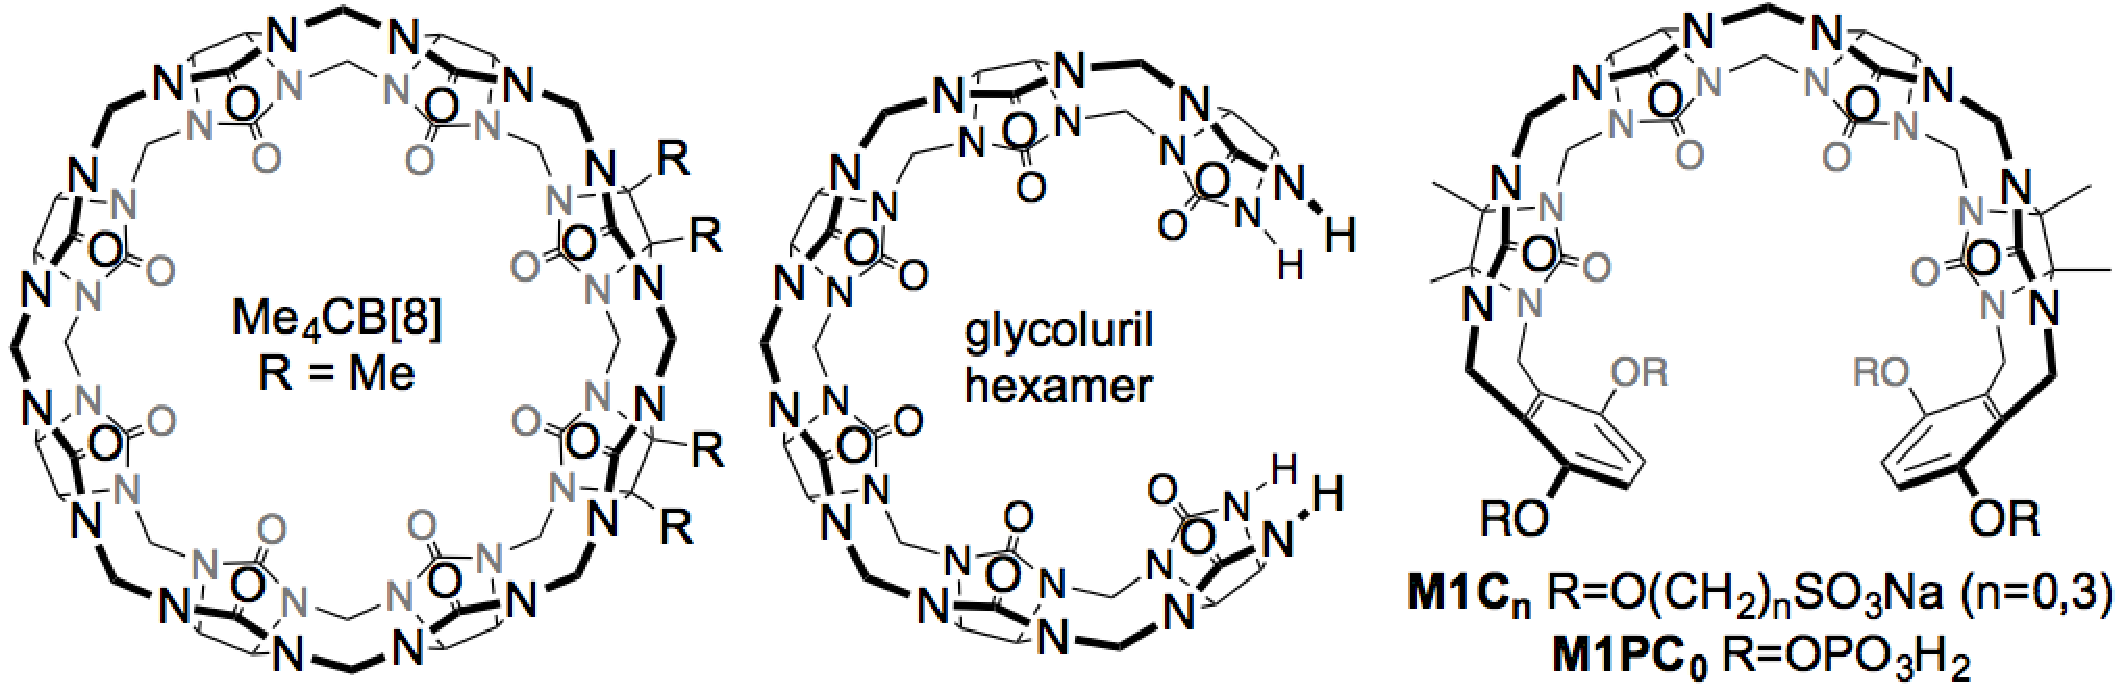
\includegraphics{figures/CB.pdf}}

\end{centering}

\vspace{0.1in}
\caption{\footnotesize {\bf Structures of Me$_4$CB[8], glycouril hexamer, and acyclic CB[n]-type receptors.}
{\color{red}[JDC: Need a stand-alone description here so someone scanning the figures will know what is going on.}
\label{figure:CB}}
\end{figure}

\textbf{SAMPL6, 8 and 10 cucubituril challenges.} 
\emph{For SAMPL6}, we will measure $K_a$ and $\Delta H$ values, stoichiometry, and geometry for the interaction of Me4CB[8] (a soluble CB[8] derivative) with 15 guests (selected top drugs, Table CB1) by either direct or competition isothermal titration calorimetry (ITC), UV/Vis or fluorescence indicator displacement assay, or NMR competition experiments, as previously~\cite{cao_attomolar_2014, liu_cucurbituril_2005, ma_acyclic_2010, she_glycoluril-derived_2016}.  
Our selection of Me$_4$CB[8] binding to top drugs allows us to modulate the computational complexity by: 1) changing host flexibility (e.g. Me$_4$CB[8] can exhibit ellipsoidal deformation)~\cite{vinciguerra_synthesis_2015}, 2) allowing the possibility of binary or ternary (e.g. 1:1 and/or 1:2 host:guest) complexes~\cite{ko_supramolecular_2007, barrow_cucurbituril-based_2015, urbach_molecular_2011}, 3) using drugs with several potential binding epitopes to induce sampling issues.  Host:guest stoichiometry and geometry (e.g. which binding epitope is complexed) will be addressed by ITC ``n'' values, Job plots monitored by UV/Vis or NMR~\cite{connors_binding_1987}, and by 1H NMR complexation induced changes in chemical shifts~\cite{masson_cucurbituril_2012}.  
All three sets of studies will be conducted in phosphate buffered saline (pH 7.4 with physiological salt) which introduces its own complexities due to salt competition for binding~\cite{marquez_mechanism_2004, mobley_predicting_2016}. 
%Isaacs old phrasing cut/simplified by DLM: "further complexity due to competitive interaction between the C=O portals of CB[n]-type receptors and metal ions via ion-dipole interactions which reduces the observed Ka values~\cite{marquez_mechanism_2004}."
For \emph{SAMPL8}, we will focus on binding of the same 15 drugs (Table~\ref{table:CB}), but to glycoluril hexamer. 
This is an ideal next step as this host exhibits increased conformational dynamics, and influences the number and energy of solvating (and unusually coordinated) water molecules implicated in the high binding constants for CB[n]-guest complexes~\cite{biedermann_release_2012, biedermann_hydrophobic_2014}.  
The selected drugs include several with pKa values in the 3.8 to 7.4 range; given that CB[n]-type receptors (like biomolecular receptors) can induce pKa shifts in their guests of up to 4 pKa units~\cite{saleh_activation_2008, nau_deep_2011, ghosh_strategic_2012}, this will test how well models can predict these effects. 
Additionally, it will couple nicely with the focus on pKa values in Aim 1.
\emph{SAMPL10} will shift to acyclic CB[n]-type receptors (e.g. M1C$_3$, M1C$_0$, and M1PC$_0$ that contain anionic solubilizing groups attached via different linker lengths.  
As in SAMPL2, these acyclic CB[n]-type receptors introduce conformational complexity, and water interactions play a key role.
%Insert SAMPL2 ref  
Moreover, the presence of 4 anionic groups in close proximity to the cavity are expected to have a significant influence on the balance between ion-dipole interactions and the solvation of the free host.

{\bf Subaim 2.2. Gibb deep cavity cavitands for host-guest studies} 

%Gibb science

%CHODERA FEEDBACK TO INCORPORATE HERE:
%* We need to emphasize why the octa-acid system has proven to be so valuable for modelers in the introduction: What specific physical challenges does the system probe, and what have we learned? We also need to add citations to the meta-analysis and maybe even all of the papers that addressed this system. David can likely address this.
%DLM: I think the above goes in the section above that introduces Aim 2.

%* I'm a bit concerned that proposing to measure only five ligands per compound is going to be perceived as lacking in statistical power required to assess accuracy, and that this specific aspect will be a liability. Is it possible to do more than that, or would this require a significantly larger chunk of money or access to automated ITC technology? Alternatively, we can be vague about how many compounds we will use or focus on the total number of compounds across all hosts. (DLM: I should probably recast a bit somewhere to explain how much we'll learn across hosts.)

{\bf History of octa-acid SAMPL challenges.} During SAMPL4~\cite{gibb_binding_2013} and SAMPL5~\cite{sullivan_binding_2016} we focused on two hosts: the octa-acid 1 (R = H) and another octa-acid derivative with four methyl groups positioned at the portal of the binding pocket (1, R = Me). 
% Chodera suggests commenting on what specific features of these hosts were remarkable for presenting isolated challenges to quantitative predictive modeling -- sterics? Charge? Protonation state effects? DLM to add discussion here or elsewhere as appropriate.
These studies used Isothermal Titration Calorimetry (ITC) to measure the thermodynamics of (1) host 1 (R = H) complexing a range of carboxylate guests,
% Chodera asks "how many?"
and (2) the binding of carboxylate and trimethylammonium guests to both hosts (1, H = H and Me).  
In both cases $^1$H-NMR titration was also used in a confirmatory role for ITC-derived free energies of binding.  
SAMPL5 emphasized how differences in the shape of the hydrophobic pocket of the host can have a profound affect on affinity for some guests.
% Add SAMPL5 overview and experimental cites
% Comment on value to community


{\bf Novel deep cavity hosts probe the effects of binding site charge constellations.} 
For future SAMPL challenges, we will expand on the range of hosts by including 2 and 3 in our ITC studies.  
Like cavitand 1, host 2 is an octa-acid derivative.  However, the four benzoate groups are relocated from the extreme exterior in the case of 1, to the rim of the binding pocket in 2.  
We surmise that this will have a direct effect on the binding of charged guests, but more subtly, an indirect effect on guest complexation via changes to the solvation of the empty host.  
Octa-trimethylammonuim cavitand (``positand'' 3) has the same overall architecture as host 1, but inverts the charges on the water solubilizing exterior coat.  While it is not yet clear if this switch in groups relatively remote from the pocket will directly affect guest complexation, results from related systems suggest it can (unpublished).

Guests for the five proposed ITC studies will be obtained from commercial sources, focusing on molecules that probe the limitations of current force-fields as well as new data as it is gathered.   
%JDC asks: "Is it worth noting the guests likely have to be highly soluble?"
% JDC asks whether we should try to pre-calculate guest affinities to aid in selecting those with a large dynamic range or large differences between host variants. I think probably we should propose this -- if we have someone working on SAMPL full-time (Aim 4) this would be very much within what we can do. I'll add something along these lines in edits.

{\bf SAMPL6-10 deep cavity cavitand challenges.} 
The host-guest challenge for SAMPL6 will focus on how well the effect of host carboxylate substituent location can be predicted, and will involve hosts 1 and 2 with a set of five, previously uninvestigated guests.  
SAMPL7 will provide a second iteration of this experiment to test algorithmic improvements in predictive modeling following SAMPL6 by comparing hosts 1 and 3 with a different set of guests.  
We anticipate that because of the relative remoteness of the charged groups in these two hosts, the effects of switching charges will be subtler than the differences between 1 and 2.  
SAMPL8 will consider the effect of common biologically-relevant counterions/salts salts on guest binding, comparing the effects of NaCl and NaI on the complexation of five guests to 1.  
We have previously shown that iodide has a weak affinity for the binding pocket of 1, whilst sodium ions have an affinity for the outer carboxylates~\cite{carnegie_anion_2014}, requiring modeling to capture the differential affinities of these ions in addition to guest affinities to successfully model the observed affinities.  
SAMPL9 will follow up on this by examining the effects of these same two salts on the complexation of five guests to 3, again giving the modeling community time to incorporate algorithmic improvements following SAMPL8. 
While we have not yet quantified salt affinities to host 3, we expect the iodide to have affinity for both the pocket and the positively charged solubilizing groups.  
For SAMPL10 we will consider the effects of co-solvents on the binding of five guests to 1 and 2 to probe the effect of co-solvent competition for the binding site, as well as effects cosolvents may have in weakening the hydrophobic effect. 

\begin{figure}[h]
\begin{centering}
\resizebox{\textwidth}{!}{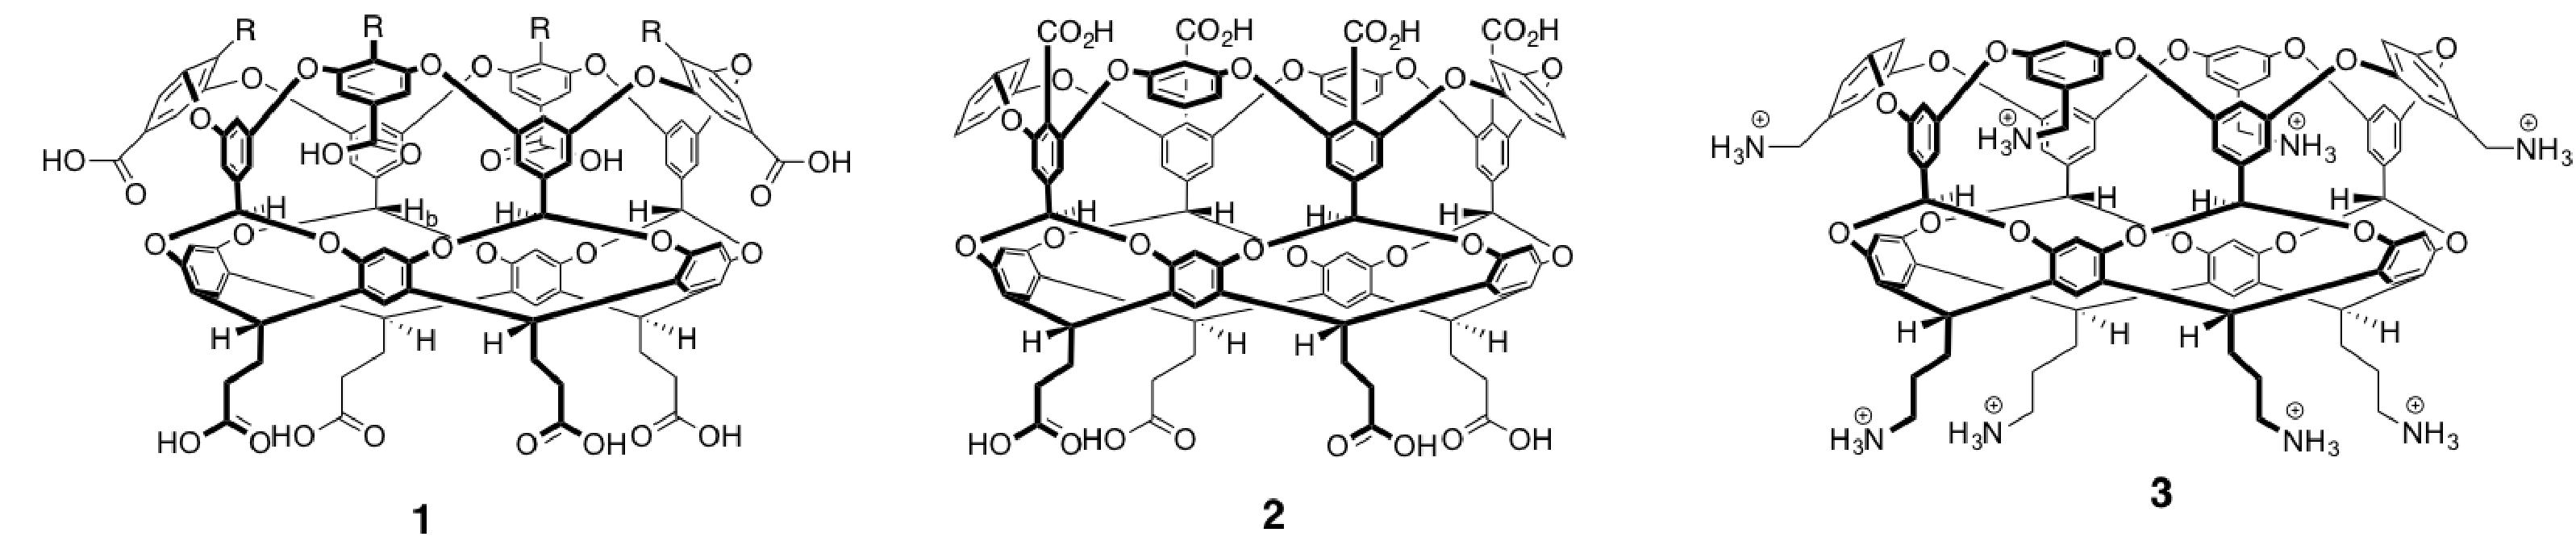
\includegraphics{figures/gdccs.pdf}}

\end{centering}

\vspace{0.1in}
\caption{\footnotesize {\bf Gibb deep cavity cavitands for SAMPL6-10.}
{\color{red}[JDC: Need a stand-alone description here so someone scanning the figures will know what is going on.}
\label{figure:gdccs}}
\end{figure}


%Aim 3 - Generate biologically relevant advanced model systems for protein-ligand binding challenges. (2 pages) 
%{\bf Aim 3. Generate biologically relevant advanced model systems for protein-ligand binding challenges.}
{\bf Aim 3. Develop model protein:ligand systems that isolate specific modeling challenges found in more complex pharmacologically relevant systems.}
A major goal of our effort is to drive advances in the quantitative modeling of protein:ligand interactions.
While the Drug Design Data Resource (D3R~\cite{gathiaka_d3r_2016}) effort provides community blind challenges for biomolecular targets of pharmaceutical interest, these targets generally contain a daunting number of complexities that frustrate the ability for current methodologies to achieve quantitative accuracy, resulting in poor performance [CITE].
For example, while kinases are targets of great interest to drug discovery, blind challenges involving kinase targets conflate issues of slow protein conformational dynamics~\cite{Lin:2013:Proc.Natl.Acad.Sci.a}, protonation state effects of both protein~\cite{Shan:2009:PNAS} and ligand~\cite{Szakacs:2005:JournalofMedicinalChemistrya,Grante:2014:SpectrochimicaActaPartA:MolecularandBiomolecularSpectroscopy}, charged ligands, and the modeling of complex divalent salt environments and phosphorylation state effects along with the standard computational challenges of conformational sampling and forcefield accuracy.
While the value of these exercises as an accurate prospective benchmark of current-generation model accuracy is unquestionable, {\bf the ability of blind challenges on complex pharmaceutical targets to rapidly advance the field of quantitative predictive modeling is limited.}

Instead, {\bf our philosophy is to identify model protein:ligand systems with the goal of \emph{isolating} individual accuracy-limiting effects in iterative cycles of prospective blind community challenges.}
This process focuses the field on identifying and evaluating multiple solutions to the accuracy-limiting effects (such as how to deal with ligand and protein protonation-state issues~\cite{Onufriev:2013:QuarterlyReviewsofBiophysics}, slow protein conformational dynamics, etc.) free from other complicating factors, allowing a direct evaluation of how well the phenomena of interest are modeled.
Datasets collected for these blind challenges then become standard benchmark datasets for retrospectively examining the effectiveness of modeling approaches in treating these effects to facilitate comparisons of methodologies in publications, while future iterations or variations of the same SAMPL experiment allow iterative refinement and prospective blinded evaluations of methodologies.
In this way, this cycle of blind challenges utilizing model systems can rapidly drive progress in rapidly overcoming scientific hurdles limiting quantitative accuracy.

While model protein-ligand systems have a long and storied history of driving progress in individual research laboratories (such as the Shoichet T4 lysozyme mutants~\cite{shoichet}), their power in blind community challenge cycles is amplified by leveraging community participation.
An excellent example of this was the collection of a challenge dataset featuring the binding of small, rigid charged molecules to bovine trypsin for SAMPL3~\cite{Newman:2011:JComputAidedMolDes}, which rapidly focused the field on the deficiencies of current alchemical free energy methodologies in treating the binding of charged ligands.
Within two years, multiple laboratories had developed and disseminated convergent practical solutions to effectively handle charged ligand binding that are now adopted as best practices~\cite{Rocklin:2013:TheJournalofChemicalPhysicsb,Reif:2014:JournalofComputationalChemistrya}.

{\bf SAMPL6-10 model protein:ligand challenges.} For the SAMPL6-10 challenges, we propose to introduce a new model protein:ligand system each year, with challenges fielded for each system for at least two consecutive years to allow iterative methodology improvement and assessment.
Immediately following the challenge, challenge data (including all primary data) will be published and released as a version-controlled benchmark dataset for retrospective evaluation.
The first challenge (introduced in SAMPL6) will focus on modeling the binding of small soluble drug fragments to a relatively rigid protein with multiple weak binding sites, isolating the ability of current-generation modeling approaches to model weak and multiple binding effects.
Because rapidly focusing the field on current challenges in predictive modeling requires the ability to adapt to deficiencies identified D3R/SAMPL challenges of the previous year, subsequent model systems will be rapidly identified and developed using a new informatics platform we have developed to identify tractable model systems.

%%%%%%%%%%%%%%%%%%%%%%%%%%%%%%%%%%%%%%%%%%%%%%%%%%%%%%%%%%%%%%%%%%%%%%%%%%%%%%%%
% FIGURE: HSA SAMPL6 CHALLENGE
%%%%%%%%%%%%%%%%%%%%%%%%%%%%%%%%%%%%%%%%%%%%%%%%%%%%%%%%%%%%%%%%%%%%%%%%%%%%%%%%
\begin{figure}[h]
\begin{centering}
\resizebox{\textwidth}{!}{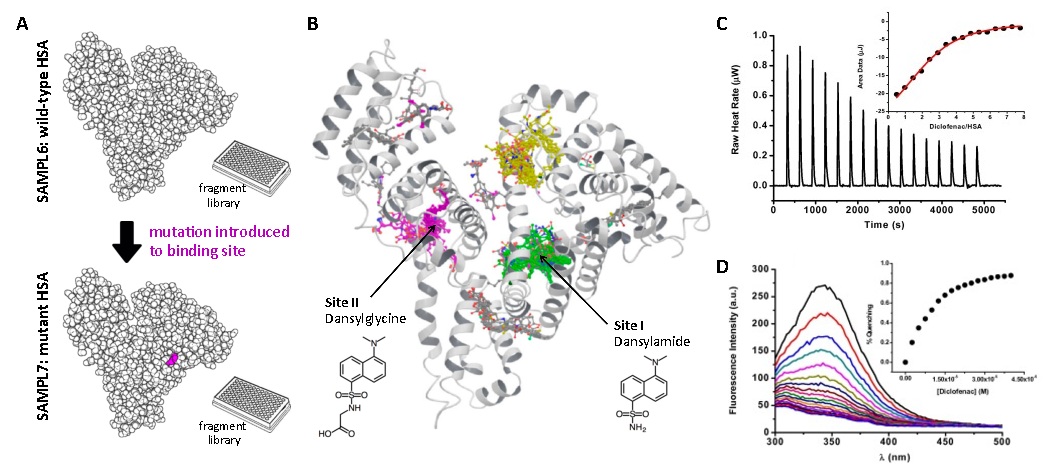
\includegraphics{figures/hsa-figure-draft4.pdf}}

\end{centering}
\vspace{0.1in}
\caption{\footnotesize {\bf The SAMPL6/7 protein:ligand challenge focuses on soluble drug fragment binding to human serum albumin (HSA).}
\emph{(A)}~SAMPL6 will introduce recombinant human serum albumin (HSA) as a target, against which a library of 96 small soluble drug fragments will be assayed.
By introducing a mutation in one of the binding pockets, we will create a second challenge target for SAMPL7.
\emph{(B)}~HSA, the most abundant plasma protein, has at least eight known binding sites, with major well-characterized sites (green, Sudlow's Site I; purple, Sudlow's Site II) observed to bind a variety of drugs, often modulating their pharmacokinetics~\cite{Fasano:2005:IUBMBLife(InternationalUnionofBiochemistryandMolecularBiology:Life)a} (figure from~\cite{Hall:2013:JournalofChemicalInformationandModelinga}).
Two fluorescent probes---dansylamide and dansylglycine---have been shown to bind with $\sim$$\mu$M affinity and high selectivity to Site I and Site II, respectively; both exhibit binding-enhanced fluorescence at 480 nm, and can be used to site-specifically probe ligand affinities by competition.
\emph{(C)}~Binding affinities of soluble molecules can easily be measured by isothermal titration calorimetry (ITC); here, the ITC titration of HSA by diclofenac (a Site II ligand~\cite{Rafols:2014:Talantaa}) is shown~\cite{Bou-Abdallah:2016:TheJournalofChemicalThermodynamics}. 
\emph{(D)}~HSA tryptophan fluorescence quenching can also be used to measure ligand binding affinity; here, HSA titration by diclofenac is shown, with the inset plot showing percent quenching at 346 nm~\cite{Bou-Abdallah:2016:TheJournalofChemicalThermodynamics}
\label{figure:hsa-challenge}}
\end{figure}
%%%%%%%%%%%%%%%%%%%%%%%%%%%%%%%%%%%%%%%%%%%%%%%%%%%%%%%%%%%%%%%%%%%%%%%%%%%%%%%%

{\bf SAMPL6: Assessing predictive modeling to multiple weak binding sites with the binding of small soluble fragments to human serum albumin (HSA).}
Human serum albumin (HSA), the most abundant blood plasma protein, has the remarkable ability to bind a great variety of small molecule drugs in multiple binding sites (Figure~\ref{figure:hsa-challenge}B)~\cite{Fasano:2005:IUBMBLife(InternationalUnionofBiochemistryandMolecularBiology:Life)a}.
As a result, HSA is not only an excellent model system for isolating the challenge of binding multiple weak ligands to a stable rigid protein, it is also a pharmacologically relevant system due to its ability to drastically modulate drug pharmacokinetics~\cite{Hall:2013:JournalofChemicalInformationandModelinga}.
HSA has at least \emph{eight} known binding sites, with numerous crystal structures available for drugs binding to two predominant sites (Sudlow Site I and II)~\cite{Hall:2013:JournalofChemicalInformationandModelinga}.
Small soluble molecules resembling drug fragments have previously been shown to have a high likelihood of detectable binding to HSA ($\ge$90\% of small druglike fragments, as detected by SPR~\cite{Elinder:2011:JournalofBiomolecularScreening}), providing an experimentally-tractable diverse set of ligands spanning several orders of magnitude in affinity [CITE].
As current advanced methodologies such as alchemical free energy calculations currently assume a single well-defined binding site with high affinity~\cite{Gilson:1997:BiophysicalJournal}, this dataset will allow the isolation of the effect of weak multiple binding from the majority of other counfounding factors in protein-ligand binding.

Recombinant HSA will be expressed in \emph{E.~coli} and purified via refolding from inclusion bodies~\cite{Latta:1987:Bio/Technology}, and will be defatted at low pH to ensure the resulting protein is free of the complications of both glycosylation and bound fatty acids found in plasma-isolated HSA~\cite{Lang:2015:BiotechnologyProgress}.
Recombinant expression will also allow a mutant form of HSA (engineered via quick-change single-primer mutagenesis) to be fielded for a SAMPL7 iteration of this challenge (Figure~\ref{figure:hsa-challenge}B).
We will obtain a diverse library of 96 soluble drug-fragment-like molecules in pre-plated format for which HSA-ligand affinities are not available in the literature as dry compound, and assay them for HSA binding using automated isothermal titration calorimetry (ITC) (Figure~\ref{figure:hsa-challenge}C), with the goal of characterizing the overall binding affinity of the compound to HSA.
%If multiple binding events can be resolved, a multi-site model will be used; otherwise, a single dominant site will be assumed.
%Participants in the blind challenge will also have the option of predicting the ITC titration curve \emph{directly}, which includes all contributions to binding to multiple sites.
The same ligands pre-plated in DMSO format will be used to conduct a separate set of fluorescence titration assays (monitoring tryptophan fluorescence quenching) and competition assays in which the site-specific fluorescent probes daynsylamide (Site I) and dansylglycine (Site II) will be used to measure site-specific affinities for Sites I and II (Figure~\ref{figure:hsa-challenge}D), allowing participants to validate whether they predicted the correct binding site and, if so, the site-specific affinity.

{\bf SAMPL7-10: Rapid, responsive development of new model systems using a novel informatics platform.}
We have developed a novel informatics platform called TargetExplorer 
%[\url{https://github.com/choderalab/targetexplorer}] 
aimed at identifying new protein targets that can be rapidly developed into experimentally- and computationally-tractable model systems focusing on individual challenges.
This tool---which will be made accessible to other laboratories via an easy-to-use web interface during the course of this project---successively filters all protein:ligand complexes identified in the PDB according to a list of criteria that allow facile development as a model protein:ligand binding system, as well as identification of systems that isolate individual challenges in modeling accuracy.
Experimental tractability includes: (1) the availability of multiple protein:ligand crystal structures; (2) known bacterial expression (e.g.~from PDB {\tt EXPRESSION\_SYSTEM} records); (3) the capacity to bind a wide dynamic range of ligands (determined via data available in ChEMBL); (4) the availability of multiple known ligands that can be purchased (via ZINC); (5) tractability of experimental affinity measurements, such as known ligands with potentially fluorescent scaffolds (for fluorescence competition assays), highly soluble ligands (for ITC), or ligands above a minimal mass (for SPR or MST).
A number of additional filters annotate potential experimentally tractable systems for suitability as a model system that isolates individual challenges, such as: charged ligands or potential ligand protonation state or tautomer~\cite{Martin:2009:JournalofComputer-AidedMolecularDesign} effects (deduced from predicted aqueous protonation/tautomer energies); potential protein protonation state effects (deduced from MCCE2 calculations~\cite{Song:2009:JournalofComputationalChemistry}); protein conformational changes (deduced from variation in protein conformation or the presence of unresolved loops in protein:ligand crystal structures); the presence of post-translational modifications that may affect affinity (deduced from Uniprot annotations); coordinated metals (identified in crystal structures); ordered waters (present in multiple crystal structures); etc.

The Chodera lab has developed an automated wetlab for the purpose of rapidly developing model protein systems using bacterial expression techniques (see Equipment and Facilities).
Potential targets matching desired challenge criteria will be screened for bacterial expression using high-throughput cloning, transformation, and expression testing, with purity and yield assessed by capillary electrophoresis on a Caliper GXII.
Targets will be screened for stability in various buffers using Thermofluor~\cite{Reinhard:2013:ActaCrystallographicaSectionFStructuralBiologyandCrystallizationCommunications}.
Ligands identified via the informatics platform to span a wide dynamic range of binding affinities will be purchased as dry powder stocks and prepared for assay by highly accurate gravimetric solution preparation techniques using a Quantos automated balance.
A wide variety of biophysical techniques are available to provide accurate, quantitative measurements of protein-ligand binding affinities, including fluorescence (if fluorescent probe ligands are available), absorption (e.g.~Soret band shifts), automated isothermal titration calorimetry (provided ligands are sufficiently soluble), surface plasmon resonance, microscale thermophoresis (MST), luminescence, and alphascreen; all except MST are fully automated.

Our approach to developing challenge datasets will be twofold:
First, small molecules similar to known ligands will be purchased and assayed, with the presumption that these molecules are likely to have measurable affinities.
Second, site-directed mutants will be introduced to modulate the binding affinities of known ligands using single-primer quick-change mutagenesis, which can be performed and screened for expression in 96-well format.
Challenge datasets will therefore consist of a matrix of protein mutants and ligands, providing a rich dataset to deeply explore the effects of interest.

%We will identify suitable biological protein-ligand model systems (difficult but tractable in order to push the limits of physical techniques) then measure binding and develop these for blind challenges. This will include binding studies on human serum albumin and bromodomains or aspartyl proteases; initial binding data will be expanded by the selection of additional ligands or the creation of mutations in the protein that modulate binding.

%%%%%%%%%%%%%%%%%%%%%%%%%%%%%%%%%%%%%%%%%%%%%%%%%%%%%%%%%%%%%%%%%%%%%%%%%%%%%%%%
% FIGURE: MODEL SYSTEM MINING
%%%%%%%%%%%%%%%%%%%%%%%%%%%%%%%%%%%%%%%%%%%%%%%%%%%%%%%%%%%%%%%%%%%%%%%%%%%%%%%%
\begin{figure}[h]
\begin{centering}
\resizebox{!}{2in}{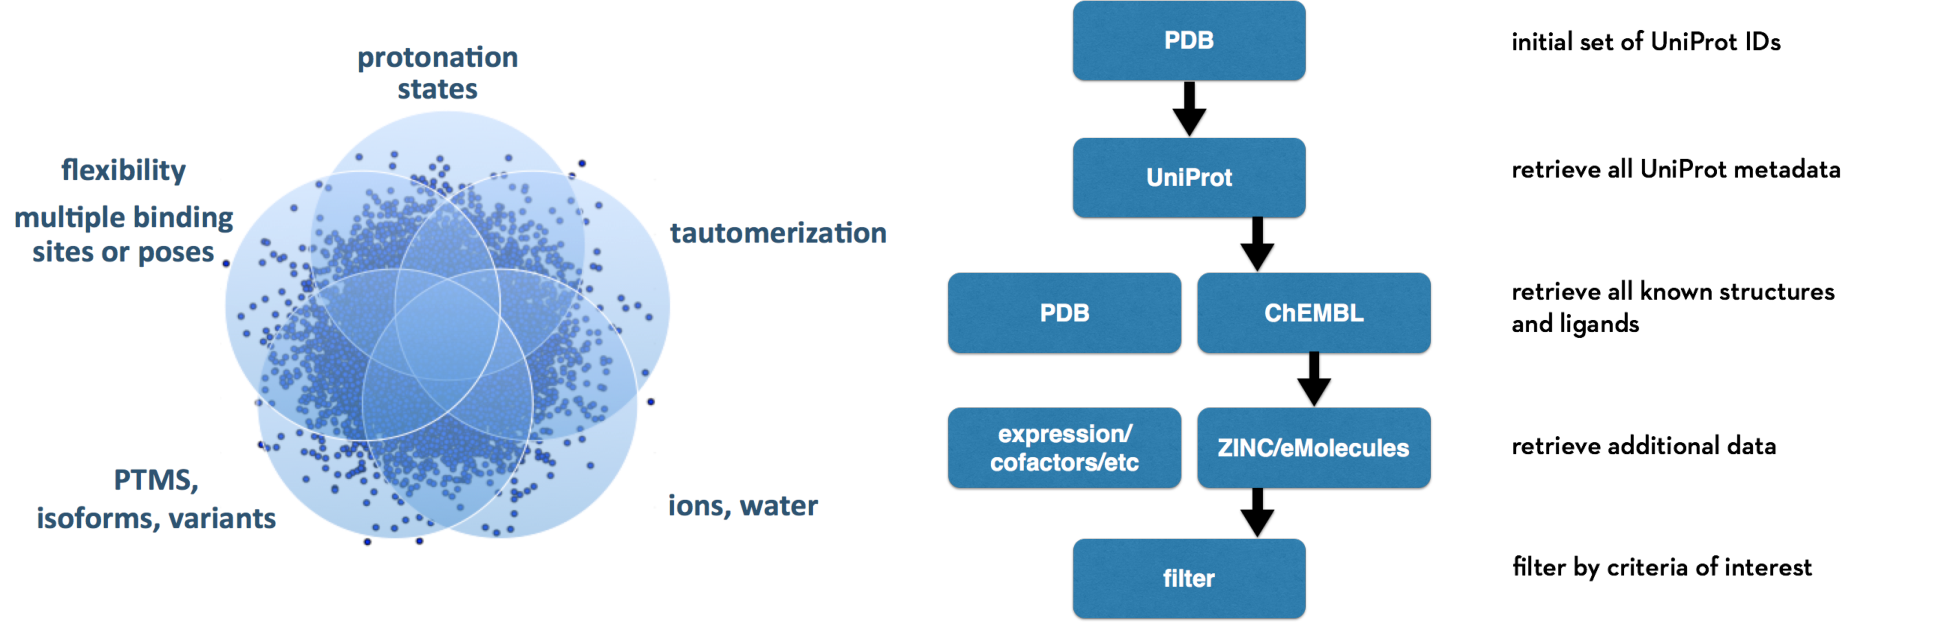
\includegraphics{figures/mining-model-systems.pdf}}

\end{centering}
\vspace{0.1in}
\caption{\footnotesize {\bf Mining model protein:ligand systems to focus on individual modeling challenges via a structural and chemical informatics platform.}
SAMPL7-10 will feature the introduction of new model protein:ligand systems designed to focus on individual challenges judged to be of critical immediate importance following current D3R/SAMPL blind competitions.
\emph{Left:} Since most protein targets of pharmaceutical interest feature a multitude of conflated challenges to quantitative accuracy, our goal is to identify model protein targets that isolate individual effects to focus community efforts by fielding new blind challenges.
\emph{Right:} In order to rapidly develop new experimentally- and computationally-tractable model protein:ligand systems, we have developed a structural and chemical informatics system that applies successive filters to the set of \emph{all} potential protein:ligand systems for which structural data is available.
{\color{red}[JDC: This figure is a placeholder.]}
\label{figure:mining-for-model-systems}}
\end{figure}
%%%%%%%%%%%%%%%%%%%%%%%%%%%%%%%%%%%%%%%%%%%%%%%%%%%%%%%%%%%%%%%%%%%%%%%%%%%%%%%%



%Aim 4 - Coordinate, run, and analyze blind challenges to advance modeling of binding (1.5 pages)
{\bf Aim 4. Coordinate, run, and analyze blind challenges to advance modeling of binding.}
The data collected in Aims 1-3 will drive annual SAMPL blind challenges, allowing the field to test the latest methods and force fields to assess progress, compare them against one another head-to-head, and perform sensitivity analysis to learn how much different factors (protonation state, tautomer selection, solvent model, force field, sampling method, etc.) affect predictive power. Results will then feed back into improved treatment of these factors for subsequent challenges, driving regular cycles of application, learning, and advancement.
%Coordinate and run SAMPL blind challenges
	%Run reference calculations to:
		%a. Test current standard methods/FF
		%b. Facilitate others learning (swap method or FF)
		%c. Do sensitivity analysis (learn what?s important)
		%d. (Give examples of what we?ve learned from this)
		%e. (We will make inputs, outputs, and methods available too)
	%Select and announce null models, run them
	%Do statistical analysis of results (& compare to nulls), report back
	%Work with D3R on meeting coordination
	%Coordinate follow-up experiments as needed (cite examples when this was desirable)
	%Coordinate with JCAMD on special issues
	%Data archival and dissemination
	%   Probably also should comment on archiving/disseminating OLD SAMPL data, which we haven't been able to do (lack of resources)
	%D3R coordination:
	%	a. Co-running workshops with D3R
	%     b. Coordinating challenges with them, submission deadlines offset from D3R challenges



%%%%%%%%%%%%%%%%%%%%%%%%%%%%%%%%%%%%%%%%%%%%%%%%%%%%%%%%%%%%%%%%%%%%%%%%%%%%%%%%%%%%%%%%%%%%%%%%%%%%%%
% TIMELINE
%%%%%%%%%%%%%%%%%%%%%%%%%%%%%%%%%%%%%%%%%%%%%%%%%%%%%%%%%%%%%%%%%%%%%%%%%%%%%%%%%%%%%%%%%%%%%%%%%%%%%%

{\bf \large TIMELINE} %1 page minus a paragraph
%"The timeline is actually likely to be very important here, so I'd strongly suggest we include it, if not expand it to one full page. We have to "sell" the reviewers on how the concept would play out into actual challenges, advances, etc. so that they get a concrete idea of all the good things that will come of this. We should mention when we would hold blind challenges, when data would be released, when meetings would occur, when benchmarks would be published, and what datasets would be generated for the community."



%%%%%%%%%%%%%%%%%%%%%%%%%%%%%%%%%%%%%%%%%%%%%%%%%%%%%%%%%%%%%%%%%%%%%%%%%%%%%%%%
% FIGURE: AIMS OVERVIEW
%%%%%%%%%%%%%%%%%%%%%%%%%%%%%%%%%%%%%%%%%%%%%%%%%%%%%%%%%%%%%%%%%%%%%%%%%%%%%%%%
%\begin{figure}[h]
%\begin{centering}
%\resizebox{\textwidth}{!}{\includegraphics{figures/timeline.pdf}}

%\end{centering}
%\vspace{0.1in}
%\caption{\footnotesize {\bf Timeline.}
%\label{figure:aims-overview}}
%\end{figure}
%%%%%%%%%%%%%%%%%%%%%%%%%%%%%%%%%%%%%%%%%%%%%%%%%%%%%%%%%%%%%%%%%%%%%%%%%%%%%%%%

%%%%%%%%%%%%%%%%%%%%%%%%%%%%%%%%%%%%%%%%%%%%%%%%%%%%%%%%%%%%%%%%%%%%%%%%%%%%%%%%%%%%%%%%%%%%%%%%%%%%%%
% COLLABORATION MANAGEMENT PLAN
%%%%%%%%%%%%%%%%%%%%%%%%%%%%%%%%%%%%%%%%%%%%%%%%%%%%%%%%%%%%%%%%%%%%%%%%%%%%%%%%%%%%%%%%%%%%%%%%%%%%%%

{\large \bf COLLABORATION MANAGEMENT PLAN} % 1 paragraph


{\large \bf OUTLOOK} %or conclusions. 0.5 page


%%%%%%%%%%%%%%%%%%%%%%%%%%%%%%%%%%%%%%%%%%%%%%%%%%%%%%%%%%%%%%%%%%%%%%%%%%%%%%%%%%%%%%%%%%%%%%%%%%%%%%
% BIBLIOGRAPHY
%%%%%%%%%%%%%%%%%%%%%%%%%%%%%%%%%%%%%%%%%%%%%%%%%%%%%%%%%%%%%%%%%%%%%%%%%%%%%%%%%%%%%%%%%%%%%%%%%%%%%%

\eject

%\footnotesize
%\scriptsize
%\bibliographystyle{acm}
\bibliographystyle{nci}
%\bibliographystyle{nar}
\bibliography{sampl-r01}

\end{document}